%% ENSF 612 Project Proposal (Revised): DupHunter
\documentclass[11pt,a4paper]{article}

\usepackage[left=2cm,right=2cm,top=1.4cm,bottom=1.6cm]{geometry}
\usepackage[T1]{fontenc}
\usepackage{lmodern}
\usepackage{microtype}
\usepackage{booktabs}
\usepackage{tabularx}
\usepackage{array}
\usepackage[table]{xcolor}
\usepackage{tikz}
\usetikzlibrary{arrows.meta}
\usepackage{enumitem}
\usepackage{multicol}
\usepackage{float}
\setlist{nosep,leftmargin=*}
\usepackage[font=small,labelfont=bf,skip=3pt]{caption}
\usepackage{titlesec}
\titlespacing*{\section}{0pt}{6pt}{2pt}
\titleformat*{\section}{\large\bfseries}
\usepackage[colorlinks=true,linkcolor=blue!50!black,citecolor=blue!50!black,urlcolor=blue!50!black]{hyperref}

\setlength{\parskip}{4pt}
\setlength{\parindent}{0pt}
\setlength{\textfloatsep}{6pt}
\setlength{\intextsep}{6pt}
\newcolumntype{Y}{>{\raggedright\arraybackslash}X}
\newcommand{\g}{\cellcolor{blue!22}}
\newcommand{\ms}{\cellcolor{orange!45}}

\begin{document}

\begin{center}
  {\Large\bfseries ENSF~612 Project Proposal (Milestone~1, Revised)}\\[3pt]
  {\small Engineering Large-Scale Data Analytics Systems, Fall 2026\\[1pt]
  Instructor: Dr.~Ebrahim Karami\\[1pt]
  October 25, 2026}
\end{center}

%% ==========================================================================
\section{Project Title}
\textbf{DupHunter: Scalable Duplicate Question Detection on Stack Overflow}

%% ==========================================================================
\section{Group Members}
{\small
\begin{tabularx}{\textwidth}{@{}l Y@{}}
\toprule
\textbf{Name} & \textbf{Main role} \\
\midrule
Satyam Bhanot & Data pipeline, Spark cluster setup, scaling experiments \\
Iesrat Jahan & Duplicate detection core: shingling, MinHash, LSH, LSH settings study \\
Md Jubayer Khan & Baselines and accuracy evaluation; SON tag blocking \\
Navjot Singh Shienh & AI-impact analysis on duplicates; streaming duplicate check \\
\bottomrule
\end{tabularx}}

%% ==========================================================================
\section{Problem Statement}

Stack Overflow is a website where programmers ask and answer questions. Many
new questions have already been asked before, just in different words. These
are called \emph{duplicates}. Today, volunteers find and close them by hand,
and many are missed.

We want to build a system that finds duplicate questions automatically. The
hard part is size. Stack Overflow has about 24 million questions, and comparing
every question with every other one would take years on one computer. We need
methods built for large data that can run on more than one machine.

Duplicate detection is the core of this project. Every other part either
improves it or uses its results.

\textbf{Questions we want to answer:}
\begin{enumerate}[label=\textbf{Q\arabic*.},leftmargin=2.2em]
  \item \textbf{(Core)} How many known duplicates can MinHash and LSH find, and
        how much comparison work does it save compared with checking every pair?
  \item \textbf{(Core)} How does the system scale with more cores, a second
        machine, and more data, and what slows it down?
  \item Does grouping questions by frequent tag sets before LSH make it faster
        without losing many duplicates?
  \item Did the share of new questions that are near-duplicates change after AI
        tools such as GitHub Copilot and ChatGPT became popular in 2022?
\end{enumerate}

\textbf{Expected outcome:} a working Spark pipeline for duplicate detection,
with measured accuracy and speed, plus two smaller studies built on top of it.

%% ==========================================================================
\section{Motivation and Application}

Duplicate questions waste time. People wait for answers that already exist,
experts answer the same thing again, and volunteers spend hours searching. A
tool that finds duplicates could show a user an existing answer before they
post. The same methods are used to remove repeated pages from web search and
from AI training data.

AI tools also changed how people use Stack Overflow. A 2024 study found that
activity dropped after ChatGPT was released~\cite{delrio2024}. We want to see
whether the questions that are still asked have become more or less repetitive.

The project fits ENSF~612 because it needs the course's tools for large data:
MapReduce and Spark, similarity search, frequent itemsets, and stream
algorithms~\cite{mmds}.

%% ==========================================================================
\section{Dataset}

\textbf{Source.} We will use the public Stack Exchange data dump on the Internet
Archive (\url{https://archive.org/details/stackexchange}). The newest release
is from September 30, 2026~\cite{sedump}. It is free to use under the
CC~BY-SA~4.0 license.

\textbf{Size and format.} The Stack Overflow archive is a single 64.2\,GiB
(68.9\,GB) compressed file (\texttt{.7z}) covering July 2008 to September 2026.
Inside, each table is an XML file with one record per line. We only need the
two tables in Table~\ref{tab:data}. Record counts are estimates from older
releases; we will update them after loading the data.

\begin{table}[H]
\centering
\caption{The data we will use.}
\label{tab:data}
\small
\begin{tabularx}{\textwidth}{@{}l l Y Y@{}}
\toprule
\textbf{Table} & \textbf{Records (approx.)} & \textbf{Fields we keep} & \textbf{What we use it for} \\
\midrule
Posts     & 60 million (24 million questions) & id, type, title, body, tags, date, author & Question text for the subset; dates and tags for all questions \\
PostLinks & 10 million & post id, related post id, link type & Known duplicate pairs (our answer key) \\
Super User site & 1.4\,GB compressed & same tables & Testing our code \\
\bottomrule
\end{tabularx}
\end{table}

\textbf{How much data we will use.}
\begin{itemize}
  \item We keep only the columns listed above and skip every other table.
  \item Duplicate detection needs the full question text and many test runs, so
        we run it on questions tagged \texttt{python} (roughly 2 million; we
        will confirm the count). This is still large: 2 million questions make
        about 2 trillion pairs. We only score duplicate pairs where both
        questions are in the subset.
  \item Dates and tags for all 24 million questions are small. We use them for
        overall question volume in Q4.
  \item We build and debug everything on the Super User site first. It has the
        same format but is about 50 times smaller.
\end{itemize}

\textbf{Data quality and limitations.}
\begin{itemize}
  \item Question text is stored as HTML, with code mixed into the writing.
  \item Deleted posts are missing.
  \item Not every duplicate was marked by volunteers, so our answer key is
        incomplete and our precision will be a lower bound.
  \item The most recent months are incomplete, because new questions may still
        be closed as duplicates.
  \item Results on one tag may not hold for every topic.
\end{itemize}

\textbf{Preprocessing.} We extract only the two tables and read them as a
stream, so we never store hundreds of GB of unpacked XML. We keep the needed
columns and save them as Parquet (a compressed table format that Spark reads
quickly), split by year. For the subset, we remove HTML tags, keep code blocks
separate, and break each question into short groups of words called
\emph{shingles}.

%% ==========================================================================
\section{Proposed Methodology}

\begin{figure}[H]
\centering
\resizebox{\textwidth}{!}{%
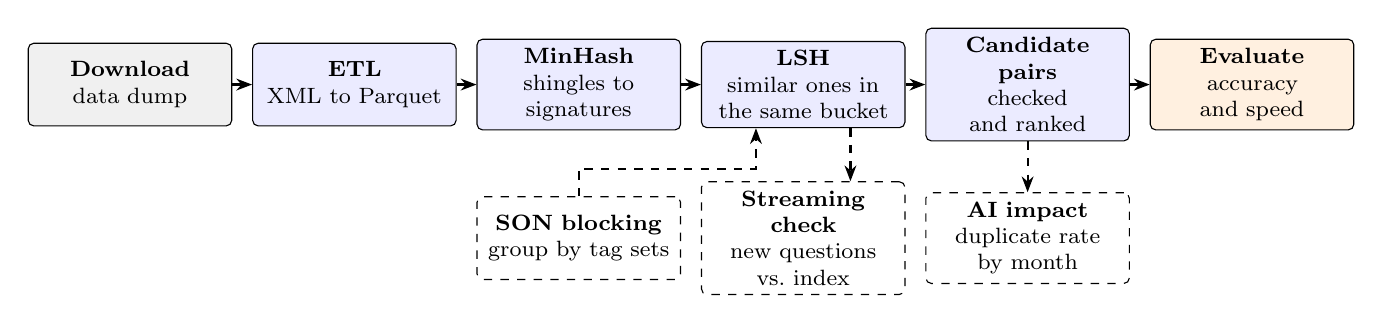
\begin{tikzpicture}[
  box/.style={draw, rounded corners=2pt, align=center, font=\footnotesize, text width=2.35cm, minimum height=1.05cm, fill=blue!8},
  side/.style={box, dashed, fill=white},
  arr/.style={-{Stealth[length=2mm]}, thick},
  darr/.style={-{Stealth[length=2mm]}, thick, dashed}
]
\node[box, fill=gray!12] (a) at (0,0)    {\textbf{Download}\\ data dump};
\node[box]               (b) at (2.85,0) {\textbf{ETL}\\ XML to Parquet};
\node[box]               (c) at (5.7,0)  {\textbf{MinHash}\\ shingles to signatures};
\node[box]               (d) at (8.55,0) {\textbf{LSH}\\ similar ones in the same bucket};
\node[box]               (e) at (11.4,0) {\textbf{Candidate pairs}\\ checked and ranked};
\node[box, fill=orange!12] (f) at (14.25,0) {\textbf{Evaluate}\\ accuracy and speed};
\draw[arr] (a) -- (b); \draw[arr] (b) -- (c); \draw[arr] (c) -- (d); \draw[arr] (d) -- (e); \draw[arr] (e) -- (f);
\node[side] (s) at (5.7,-1.95)   {\textbf{SON blocking}\\ group by tag sets};
\node[side] (t) at (8.55,-1.95)  {\textbf{Streaming check}\\ new questions vs.\ index};
\node[side] (u) at (11.4,-1.95)  {\textbf{AI impact}\\ duplicate rate by month};
\draw[darr] (s.north) -- ++(0,0.35) -| ([xshift=-6mm]d.south); \draw[darr] ([xshift=6mm]d.south) -- ([xshift=6mm]t.north); \draw[darr] (e.south) -- (u.north);
\end{tikzpicture}}
\caption{DupHunter pipeline. The top row is the core. Dashed boxes are the secondary parts.}
\label{fig:pipeline}
\end{figure}

\textbf{Core: duplicate detection (Q1).} We turn each question into shingles
and compress them into a short MinHash \emph{signature}. LSH then puts similar
signatures into the same bucket, and we only compare questions that share a
bucket. We will try several LSH settings (numbers of bands and rows), because
too few bands miss duplicates and too many give false matches.

\textbf{Secondary parts, all built on the core.}
\begin{itemize}
  \item \textbf{SON tag blocking (Q3).} Find frequent tag sets with the SON
        algorithm, then run LSH separately inside each tag group. We measure
        how much faster this is and how many duplicates it loses.
  \item \textbf{AI impact (Q4).} Use the duplicates found by the core to
        compute the monthly share of new questions that are near-duplicates,
        and compare it before and after June 2022 (Copilot) and November 2022
        (ChatGPT).
  \item \textbf{Streaming check.} Replay questions in date order and check each
        new one against the LSH index as it arrives. DGIM keeps a rolling count
        of duplicates in the most recent questions, and Flajolet-Martin counts
        distinct askers. Unlike an exact Spark SQL query, which needs all the
        data stored and more memory as data grows, these answer in one pass
        with fixed memory. We will show their error for different memory sizes,
        compare their memory with the exact counts, and measure updates per
        second.
\end{itemize}

\textbf{Priority and cut order.} Q1 and Q2 must be finished. If time runs
short, we cut the streaming check first, then the AI-impact study, then SON
blocking. The core on its own still covers every guideline requirement.

\textbf{Compute setup.} We have two laptops, each with an Intel Core i7 and
16\,GB of RAM. We will connect them as a Spark standalone
cluster~\cite{zaharia2012}: Laptop~A runs the master, the driver, and one
worker; Laptop~B runs one worker. Each worker gets about 8 cores and 10\,GB of
memory. MinHash signatures for 2 million questions need only about 1\,GB, so
this is enough. Both laptops will be on the same wired network, so that moving
data between them does not dominate the timings. The laptops also have NVIDIA
GPUs, which we will not use, because the course algorithms do not need them.

\textbf{How we will evaluate.}
\begin{itemize}
  \item \textbf{Accuracy (Q1):} Recall@K, Precision@K, MAP (how high real
        duplicates rank), and reduction ratio (the share of pairs we never
        compare). Baselines: an exact all-pairs check on a sample of 100{,}000
        questions, and Spark's built-in \texttt{MinHashLSH}.
  \item \textbf{Blocking (Q3):} run time, data moved between machines, and
        recall, with and without SON blocking.
  \item \textbf{AI impact (Q4):} monthly duplicate share and question volume,
        before and after 2022.
  \item \textbf{Scaling (Q2):} the three tests in Table~\ref{tab:scale}. For
        each run we record run time, speedup (how many times faster it is than
        with one core), data moved between machines, and peak memory. Each
        setting runs three times.
\end{itemize}

\begin{table}[H]
\centering
\caption{Scaling tests on the two-laptop cluster.}
\label{tab:scale}
\small
\begin{tabularx}{\textwidth}{@{}l Y Y@{}}
\toprule
\textbf{Test} & \textbf{Setup} & \textbf{What it shows} \\
\midrule
A. More cores & 1, 2, 4, and 8 cores on one laptop; same data & Speedup from adding cores \\
B. Second machine & 8 cores on one laptop vs.\ 4 + 4 on two laptops; then 8 + 8 & The cost of sending data over the network \\
C. More data & 10\%, 25\%, 50\%, and 100\% of the subset on both laptops & How run time grows with data size \\
\bottomrule
\end{tabularx}
\end{table}

%% ==========================================================================
\section{Algorithms and Techniques}

We write the course algorithms ourselves and compare them with ready-made tools,
so the report clearly shows which code is ours.

\begin{table}[H]
\centering
\caption{Algorithms, baselines, and priority.}
\label{tab:alg}
\small
\begin{tabularx}{\textwidth}{@{}Y Y l l@{}}
\toprule
\textbf{Our own code} & \textbf{Compared with} & \textbf{Priority} & \textbf{Q} \\
\midrule
Shingling, MinHash, LSH~\cite{broder1997,indyk1998} in Spark & Exact check on a sample; Spark \texttt{MinHashLSH} & Core & Q1 \\
Spark jobs in the MapReduce style~\cite{dean2004} & Same jobs with fewer cores or one machine & Core & Q2 \\
SON frequent itemsets~\cite{son1995} for tag blocking & LSH without blocking; Spark \texttt{FPGrowth} & Secondary & Q3 \\
Monthly before/after comparison of duplicate share & Same months before 2022 & Secondary & Q4 \\
DGIM~\cite{dgim2002}, Flajolet-Martin~\cite{fm1985} in a streaming check & Exact counts in Spark SQL & Cut first & Q1 \\
\bottomrule
\end{tabularx}
\end{table}

%% ==========================================================================
\section{Expected Challenges}
{\small
\begin{tabularx}{\textwidth}{@{}p{6.6cm} Y@{}}
\toprule
\textbf{Challenge} & \textbf{How we plan to handle it} \\
\midrule
Duplicates written in very different words & Measure how recall changes with similarity; note it as a limit of word-based shingles \\
Missing duplicate labels & Treat precision as a lower bound; rely mainly on recall \\
Some LSH buckets become huge (common phrases) & Limit bucket size and split large buckets \\
Choosing LSH settings & Test several band and row settings on Super User first \\
Moving data between the two laptops & Wired network; process LSH buckets in batches; measure data moved \\
16\,GB of memory per laptop & Keep only needed columns; keep large results on disk; use the subset \\
Blocking misses duplicates with different tags & Measure the recall lost compared with no blocking \\
\bottomrule
\end{tabularx}}

%% ==========================================================================
\section{Expected Results}
\begin{itemize}
  \item \textbf{Q1:} LSH will find most known duplicates while skipping more
        than 99.9\% of all question pairs, and our version will perform close to
        Spark's built-in one.
  \item \textbf{Q2:} adding cores will help most for MinHash, which needs no
        communication. The second laptop will help less for LSH, because data
        must move over the network.
  \item \textbf{Q3:} tag blocking will cut run time and data moved, with a
        small loss in recall.
  \item \textbf{Q4:} the share of near-duplicate questions will change after
        2022; we expect a drop in simple, repeated questions.
\end{itemize}

%% ==========================================================================
\section{Initial Project Schedule}

The core comes first. On November 13 we check progress and decide whether the
secondary parts go ahead.

\begin{table}[H]
\centering
\caption{Weekly plan (blue: main work; orange: milestone).}
\label{tab:plan}
\footnotesize
\setlength{\tabcolsep}{3pt}
\begin{tabularx}{\textwidth}{@{}Y l *{6}{>{\centering\arraybackslash}p{1.3cm}}}
\toprule
\textbf{Task (week starting)} & \textbf{Who} & \textbf{Oct 26} & \textbf{Nov 2} & \textbf{Nov 9} & \textbf{Nov 16} & \textbf{Nov 23} & \textbf{Nov 30} \\
\midrule
Download, ETL, cluster setup          & Satyam  & \g & \g &  &  &  &  \\
MinHash and LSH, settings study       & Iesrat  & \g & \g & \g &  &  &  \\
Baselines and accuracy evaluation     & Jubayer &  & \g & \g &  &  &  \\
Core checkpoint                       & All     &  &  & \ms Nov 13 &  &  &  \\
Scaling tests                         & Satyam  &  &  & \g & \g &  &  \\
SON tag blocking                      & Jubayer &  &  & \g & \g &  &  \\
AI impact; streaming check            & Navjot  &  & \g & \g & \g &  &  \\
Results freeze                        & All     &  &  &  & \ms Nov 20 &  &  \\
Presentation                          & All     &  &  &  & \g & \g &  \\
Final report and code                 & All     &  &  &  &  & \g & \ms Dec 4 \\
\bottomrule
\end{tabularx}
\end{table}

%% ==========================================================================
\section{References}
\vspace{-14pt}
\begin{multicols}{2}
{\footnotesize
\renewcommand{\section}[2]{}
\begin{thebibliography}{99}
\setlength{\itemsep}{0pt}
\setlength{\parskip}{0pt}
\bibitem{mmds} A.~Rajaraman and J.~D.~Ullman, \emph{Mining of Massive Datasets}. Cambridge University Press, 2011.
\bibitem{sedump} Stack Exchange, Inc., ``Stack Exchange Data Dump 2026-09-30,'' Internet Archive, \url{https://archive.org/details/stackexchange_20260930}.
\bibitem{delrio2024} R.~M.~del Rio-Chanona, N.~Laurentsyeva, and J.~Wachs, ``Large language models reduce public knowledge sharing on online Q\&A platforms,'' \emph{PNAS Nexus}, vol.~3, no.~9, 2024.
\bibitem{dean2004} J.~Dean and S.~Ghemawat, ``MapReduce: Simplified data processing on large clusters,'' in \emph{Proc. OSDI}, 2004.
\bibitem{zaharia2012} M.~Zaharia \emph{et al.}, ``Resilient distributed datasets: A fault-tolerant abstraction for in-memory cluster computing,'' in \emph{Proc. NSDI}, 2012.
\bibitem{broder1997} A.~Z.~Broder, ``On the resemblance and containment of documents,'' in \emph{Proc. Compression and Complexity of Sequences}, 1997.
\bibitem{indyk1998} P.~Indyk and R.~Motwani, ``Approximate nearest neighbors: Towards removing the curse of dimensionality,'' in \emph{Proc. ACM STOC}, 1998.
\bibitem{son1995} A.~Savasere, E.~Omiecinski, and S.~Navathe, ``An efficient algorithm for mining association rules in large databases,'' in \emph{Proc. VLDB}, 1995.
\bibitem{dgim2002} M.~Datar, A.~Gionis, P.~Indyk, and R.~Motwani, ``Maintaining stream statistics over sliding windows,'' \emph{SIAM J. Comput.}, vol.~31, no.~6, 2002.
\bibitem{fm1985} P.~Flajolet and G.~N.~Martin, ``Probabilistic counting algorithms for data base applications,'' \emph{J. Comput. Syst. Sci.}, vol.~31, no.~2, 1985.
\end{thebibliography}}
\end{multicols}

\end{document}
